% Dies ist die Hauptdatei, von der aus das Gesamtdokument erzeugt wird.  Diese
% Datei sollten Sie zunächst umbenennen, damit sie keinen generischen Namen
% hat!  Dann wird sie mit LuaLaTeX kompiliert.

% In der Datei defs.tex werden alle globalen LaTeX-spezifischen Einstellungen
% vorgenommen
% Jede LaTeX-Datei beginnt mit der Dokumentenklasse.  Für diese Vorlage wurde
% die Klasse "scrreprt" von KOMA-Script gewählt, die in etwa der
% Standardklasse "report" entspricht, allerdings wesentlich mehr Möglichkeiten
% bietet und im gewissen "moderner" ist.  Eine sehr ausführliche Dokumentation
% zu KOMA-Script findet man unter der folgenden Adresse:
% http://mirrors.ctan.org/macros/latex/contrib/koma-script/doc/scrguide.pdf
\documentclass[
  % die Schriftgröße - sollten Sie nicht ändern
  fontsize=12pt,
  % das Papierformat, also DIN A4
  paper=A4,
  % Literaturverzeichnis ins Inhaltsverzeichnis
  bibliography=totoc,
  % andere Verzeichnisse ebenfalls ins Inhaltsverzeichnis
  listof=totoc,
  % abgesetzte Formeln linksbündig
  fleqn,
  % für die Satzspiegelkonstruktion - siehe KOMA-Doku
  DIV=12,
  % Bindekorrektur (linker Rand) - evtl. anpassen
  BCOR=1mm,
  % die im Text verwendeten Sprachen (u.a. für das Paket babel); die
  % letztgenannte (!) Sprache ist die Standardsprache; "n"german steht für die
  % neue Rechtschreibung
  english,ngerman,
  % weil (s.u.) das Paket geometr verwendet wird
  usegeometry,
  % wie Absätze gesetzt werden: ohne Einzug, halbe Zeile Abstand
  parskip=half-
]{scrreprt}

% Beschriftungen für Tabellen kommen linksbündig über die Tabelle
\KOMAoption{captions}{tableheading,nooneline}
\setcaptionalignment[figure]{c}
\setcaptionalignment[table]{l}

% wird für die Titelseite benötigt
\usepackage{geometry}

% Standardpaket für Lokalisation, siehe Option "ngerman" oben
\usepackage{babel}
% Laden von optimierten Trennmustern
\babelprovide[hyphenrules=ngerman-x-latest]{ngerman}

% Standardpaket für mathematische Zusatzfunktionen; wenn Sie keine
% mathematischen Formeln brauchen, können Sie diese Zeile löschen
\usepackage{amsmath}

% die Hauptschrift Libertinus
\usepackage{libertinus-otf}
% die "Schreibmaschinenschrift" Anonymous Pro, angepasst
\usepackage{AnonymousPro}
\setmonofont{AnonymousPro}[Scale=MatchLowercase,FakeStretch=0.85]

% etwas größerer Zeilenabstand als im Buchsatz
\linespread{1.1}

% Paket für Feinkorrekturen an der Typographie, das für ein ausgewogeneres
% Schriftbild sorgt
\usepackage{microtype}

% Paket für kontextsensitive Anführungszeichen
\usepackage{csquotes}
% Shortcut, damit aus dem eigentlich falschen Zeichen " richtige
% Anführungszeichen je nach Sprache werden
\MakeOuterQuote{"}

% Paket, das den Befehl \includegraphics ermöglicht
\usepackage{graphicx}

% komfortablere Aufzählungen als in Standard-LaTeX; ein Beispiel findet man in
% chap3.tex
\usepackage{enumitem}

% Paket für mehr als die üblichen Standardfarben
\usepackage[dvipsnames]{xcolor}
% Definition der "Hausfarben" der HAW
\definecolor{haw}{HTML}{003CA0}
\definecolor{haw2}{HTML}{0096D2}
\definecolor{haw3}{HTML}{A0BEDC}

% typographisch anspruchsvolle Tabellen; siehe chap3.tex
\usepackage{booktabs}

% zum Erstellen des Literaturverzeichnisses; der gängige Stil APA ist hier
% bereits eingestellt
\usepackage[style=apa]{biblatex}
% eine Beispieldatei für ein Literaturverzeichnis
\addbibresource{demo.bib}

% für die Erzeugung der Grafiken in chap3.tex; wenn Sie PGF/TikZ nicht
% verwenden wollen, können Sie diese Zeilen entfernen
\usepackage{tikz}
% Zusatzbibliotheken für TikZ, die in den genannten Beispielen verwendet
% werden
\usetikzlibrary{calc,intersections,angles,3d}

% für die Erzeugung des Codeblocks in chap3.tex; wenn in Ihrer Arbeit keine
% Codeblöcke vorkommen, können Sie diese Zeilen entfernen
\usepackage{listings}
% Anpassung des Erscheinungsbildes des Codeblocks; mehr dazu in der
% Dokumentation des Pakets "listings"
\lstdefinestyle{mystyle}{
    backgroundcolor=\color{gray!20},
    keywordstyle=\color{haw2},
    numberstyle=\footnotesize\color{haw},
    basicstyle=\ttfamily\small,
    captionpos=t,
    frame=single,
    framerule=0pt,
    keepspaces=true,
    numbers=left,
    numbersep=6pt,
    belowcaptionskip=1em,
    aboveskip=\bigskipamount,
}
\lstset{style=mystyle}
% damit es "Codeblock" und nicht "Listing" heißt
\renewcommand{\lstlistingname}{Codeblock}

% für die Verlinkung innerhalb des PDF-Dokuments, für PDF-Lesezeichen und
% PDF-Metadaten; dieses Paket sollte üblicherweise immer als letztes geladen
% werden
\usepackage[colorlinks=true,allcolors=haw,hyperfootnotes=false,pageanchor=true,linktoc=all]{hyperref}

% für die Druckversion können Sie die obige Zeile durch die folgende ersetzen,
% damit Links nicht blau dargestellt werden:
% \usepackage[draft]{hyperref}

% Metadaten des PDF-Dokumentes; setzen Sie hier Ihren eigenen Namen sowie den
% Titel Ihrer Arbeit ein
\hypersetup{pdfauthor={Prof. Dr. Edmund Weitz}}
\hypersetup{pdftitle={Handreichung zur Formatierung von Bachelorarbeiten}}


% Wenn das Kommentarzeichen entfernt wird, kann man mit einem Befehl wie
%
% \includeonly{chap2,chap3}
%
% erreichen, dass nur ausgewählte Dateien kompiliert werden.  Das ist für die
% Arbeit an umfangreichen Dokumenten hilfreich, weil es Zeit spart.  Für das
% Erstellen des fertigen Dokuments muss der Befehl natürlich wieder
% auskommentiert werden, damit alle Referenzen aktuell sind und die
% Seitenzahlen stimmen.

% Hier beginnt das eigentliche Dokument.  Sie können weitere Dateien
% hinzufügen und natürlich auch vorhandene weglassen.  Die vorhandene
% Dateistruktur ist lediglich als Beispiel gedacht.
\begin{document}
% In dieser Umgebung wird die Titelseite separat vom restlichen Text gesetzt
\begin{titlepage}
  % andere Seitenränder als im Rest der Arbeit
  \newgeometry{lmargin=2cm,tmargin=7mm,rmargin=5mm,bmargin=1cm}
  % die "Hausfarbe" der HAW; diese und die folgenden Einstellungen sind lokal
  % und gelten nur innerhalb der Umgebung "titlepage"
  \color{haw}
  % Blocksatz für die Titelseite deaktivieren
  \raggedright
  % Logo rechtsbündig setzen
  \hfill
\includegraphics[width=7cm]{HAW_Marke_RGB_300dpi}\\

  % vertikaler Abstand
  \vspace{5cm}

  % Wahl der "Hausschrift" Open Sans der HAW, die als Schrift auf Ihrem
  % Rechner installiert sein muss
  \setmainfont{Open Sans}
  % etwas kleiner als üblich
  \small
  % fett und in Majuskeln
  \textbf{BACHELORARBEIT}

  % vertikaler Abstand
  \vspace{8mm}

  % der Titel der Arbeit als "Seite in der Seite"; natürlich müssen Sie hier
  % Ihren Titel eintragen
  \begin{minipage}{0.8\linewidth}
    % Wahle der zweiten "Hausschrift" der HAW, die ebenfalls auf Ihrem Rechner
    % bereits vorhanden sein muss
    \setmainfont{Martel Heavy}
    % ziemlich große Schrift
    \LARGE
    % [1mm] steht jeweils für einen etwas größeren Durchschuss
    Handreichung\\[1mm]
    zur Formatierung\\[1mm]
    von Bachelorarbeiten\\[1mm]
    am Department Medientechnik\\
    % am Ende noch ein waagerechter Strich, das CD will es so...
    \,\rule{11mm}{1.2mm}
  \end{minipage}

  % vertikaler Abstand, überraschenderweise
  \vspace{1cm}

  % hier korrektes Datum und Ihren Namen eingeben
  vorgelegt am 26. März 2022\\
  Marlene Mustermann

  % letzter vertikaler Abstand für heute
  \vspace{5cm}

  % noch eine "Seite in der Seite", etwas nach rechts geschoben
  \hspace*{37mm}
  \begin{minipage}{0.5\linewidth}
    % Namen und Titel der beiden Prüfer eintragen
    \begin{tabular}{@{}ll}
      Erstprüferin: & Prof. Dr. Vera Musterfrau\\[-.3mm]
      Zweitprüfer: & Prof. Dr. Heinz Musterdorf \\
    \end{tabular}\\

    % noch ein horizontaler Strich
    \,\rule{9mm}{1mm}\\[1.5mm]

    \textbf{HOCHSCHULE FÜR ANGEWANDTE}\\
    \textbf{WISSENSCHAFTEN HAMBURG}\\
    Department Medientechnik\\
    Finkenau 35\\
    22081 Hamburg
  \end{minipage}
\end{titlepage}
% setzt die Geometrie wieder auf die Standardwerte zurück
\restoregeometry

% für die Seite mit dem Abstract keine Seitenzahl ausgeben
\thispagestyle{empty}

\section*{Zusammenfassung}

% Hier ersetzen Sie bitte die vorhandenen Texte durch Ihre eigenen
% Zusammenfassungen
Der Arbeit beginnt mit einer kurzen Beschreibung ihrer zentralen Inhalte, in
der die Thematik und die wesentlichen Resultate skizziert werden.  Diese
Beschreibung muss sowohl in deutscher als auch in englischer Sprache vorliegen
und sollte eine Länge von etwa 150 bis 250 Wörtern haben.  Beide Versionen
zusammen sollten nicht mehr als eine Seite umfassen.  Die Zusammenfassung
dient u.\,a.\ der inhaltlichen Verortung im Bibliothekskatalog.

% Zum Wechseln der Sprache siehe den Kommentar in chap3.tex
{
  \begin{otherlanguage}{english}
    \section*{Abstract}

    The thesis begins with a brief summary of its main contents, outlining the
    subject matter and the essential findings.  This summary must be provided
    in German and in English and should range from 150 to 250 words in length.
    Both versions combined should not comprise more than one page.  Among
    other things, the abstract is used for library classification.
  \end{otherlanguage}
}

% In der Titelei werden römische Ziffern für die Seitenzahlen verwendet;
% gleichzeitig wird durch diesen Befehl die aktuelle Seitenzahl auf eins
% gesetzt
\pagenumbering{Roman}

% Inhaltsverzeichnis
\tableofcontents

% Abbildungsverzeichnis, kann evtl. weggelassen werden
\listoffigures

% Tabellenverzeichnis, kann evtl. weggelassen werden
\listoftables

% weitere Verzeichnisse (z.B. Codeblöcke) sind theoretisch möglich

% neue Seite, vorsichtshalber
\clearpage
% ab jetzt arabische Ziffern und wieder auf eins setzen
\pagenumbering{arabic}
\section{Einleitung}\label{sec:einleitung}
dasd \cite[]{chai_optimizing_2024}
% -*- coding: utf-8 -*-

% Ausgabe des Literaturverzeichnisses; ohne weitere Optionen werden nur die
% Bücher und Artikel ausgegeben, die in der Arbeit auch zitiert werden.
\printbibliography

% markiert den Anfang des Anhangs
\appendix

% ein Kapitel, das nicht numeriert, aber trotzdem ins Inhaltsverzeichnis
% aufgenommen wird
\clearpage
\section*{Anhang}
\begin{figure}[p]
	\centering
	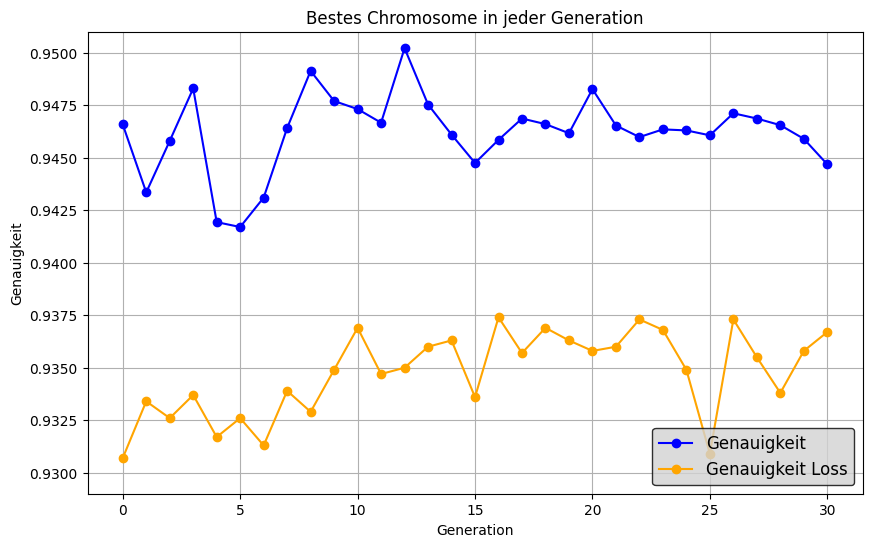
\includegraphics[width=1\linewidth]{acc.png}
	\caption{Lauf mit Priorisierung der Exploitation: Höchste Genauigkeit pro Generation}
	\label{fig:enter-label}
\end{figure}

\begin{figure}[p]
	\centering
	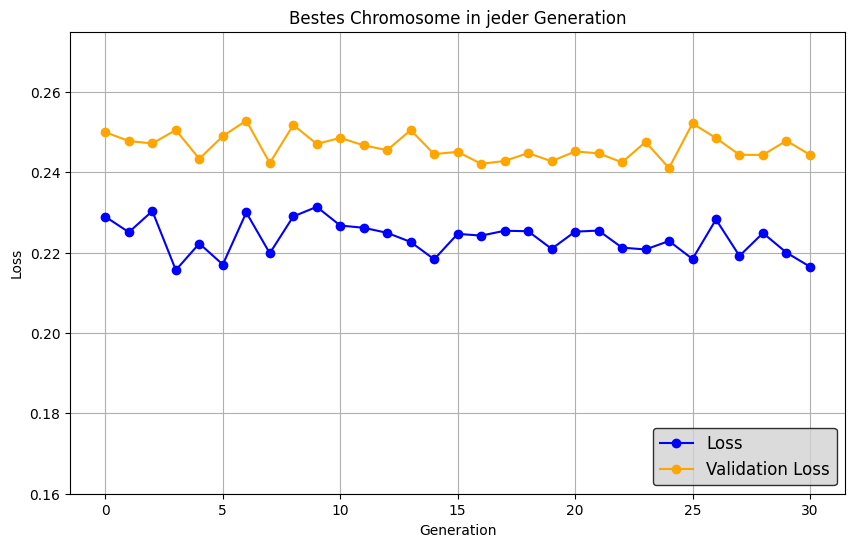
\includegraphics[width=1\linewidth]{loss_explore.png}
	\caption{Lauf mit Priorisierung der Exploration: Geringster Fehler pro Generation}
	\label{fig:enter-label}
\end{figure}

\begin{figure}[p]
	\centering
	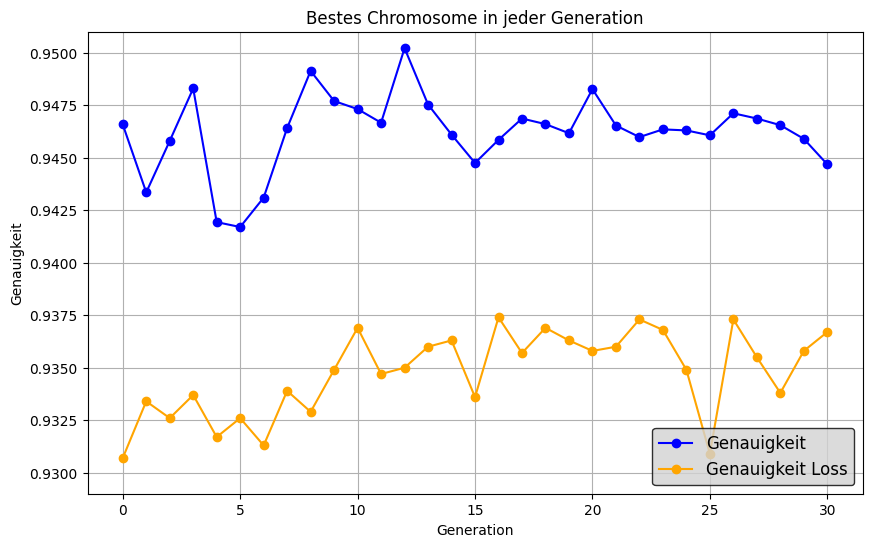
\includegraphics[width=1\linewidth]{acc.png}
	\caption{Lauf mit Priorisierung der Exploration: Höchste Genauigkeit pro Generation}
	\label{fig:enter-label}
\end{figure}


Der Sourcecode steht auf Github zur Verfügung:\\
\url{https://github.com/jonasmetzger2000/KI-STG-GI-Neural-Network-Optimizer}

% neue Seite
\clearpage

% keine Seitenzahl
\thispagestyle{empty}

% keine Nummerierung, keine Aufnahme ins Inhaltsverzeichnis
\section*{Eigenständigkeitserklärung}

% Hier müssen Sie natürlich den Titel der Arbeit sowie Ort und Datum ersetzen:
Hiermit versichere ich, dass ich die vorliegende Bachelorarbeit mit dem Titel
\begin{center}
  \textbf{Optimierung der Hyperparameter eines Neuronalen Netzes durch einen evolutionären Algorithmus}
\end{center}
selbstständig und nur mit den angegebenen Hilfsmitteln verfasst habe.  Alle
Passagen, die ich wörtlich aus der Literatur oder aus anderen Quellen wie
z.\,B. Internetseiten übernommen habe, habe ich deutlich als Zitat mit Angabe
der Quelle kenntlich gemacht.

\vspace{2cm}

Hamburg, 2. August 2024

\end{document}